% main.tex — workshop paper draft. Build: make  (pdflatex + bibtex)
\documentclass[10pt,twocolumn]{article}
\usepackage[margin=0.75in]{geometry}
\usepackage[utf8]{inputenc}
\usepackage[T1]{fontenc}
\usepackage{textcomp}
\usepackage{mathptmx}
\usepackage{amsmath,amssymb}
\usepackage{booktabs}
\usepackage{graphicx}
\usepackage{microtype}
\usepackage{url}
\usepackage[hidelinks]{hyperref}

\title{When Does Erasure Coding Beat Retransmission for RDMA?\\
\large Decode Cost Decides at Microsecond RTTs}
\author{Ibrahim Mammadov\\
ZJU-UIUC Institute, Zhejiang University\\
\texttt{ibrahimmemmedov9a@gmail.com}}
\date{}

\begin{document}
\maketitle

\begin{abstract}
Forward erasure coding (FEC) can hide packet loss from RDMA transfers without waiting for a
retransmission. Recent work shows it beats selective repeat over long-haul links with millisecond
round-trip times (RTTs), but it does not account for the cost of decoding. Inside a datacenter,
RTTs are a few microseconds, so decoding time competes directly with recovery by retransmission.
We measure this cost and its effect. Intel ISA-L, a widely deployed Reed--Solomon library, inverts
a $k\times k$ matrix on every new loss pattern. On a Sapphire Rapids server this takes 21\,\textmu s
at $k{=}16$ and 160\,\textmu s at $k{=}32$. Erasure-count decoding, a known technique that inverts
only an $m'\times m'$ matrix for the $m'$ lost packets, takes 0.8--3.4\,\textmu s for up to four lost packets on the same SIMD
kernel. Using a validated discrete-event simulator, we show that this difference decides the
outcome. For a 64-flow collective step at $10^{-3}$ loss, FEC with ISA-L's decoder loses to
selective repeat with a tail-loss probe at every RTT up to 10\,\textmu s. With erasure-count
decoding it wins at every RTT, by $1.2$--$3.0\times$. The same reversal holds under bursty loss
calibrated to production measurements. The benchmark and simulator are open source.
\end{abstract}

\section{Introduction}

Large-scale training synchronises gradients with collective operations over RDMA. One step of a
collective finishes only when its slowest flow finishes, so a single lost packet can stall the
whole step. RoCE NICs recover losses by retransmission: go-back-N on commodity
hardware~\cite{rocescale,irn}, or selective repeat in proposals such as IRN~\cite{irn}. Both need
at least one RTT, and a lost \emph{final} packet triggers no out-of-order arrival, so it waits for
a timeout.

Forward erasure coding avoids the round trip by sending parity packets. SDR-RDMA~\cite{sdrrdma}
shows that erasure coding beats selective repeat for RDMA over long-haul links, where the RTT is
25\,ms. That analysis assumes encoding overlaps transmission and does not measure decoding.
Over 25\,ms RTTs that is reasonable; inside a datacenter it is not. With RTTs of a few
microseconds, a decoder that takes tens of microseconds can be slower than simply retransmitting.

This paper asks a narrower question than prior work: \emph{at intra-datacenter RTTs, does the choice
of Reed--Solomon decoder decide whether FEC beats retransmission?} We find that it does.
\begin{itemize}
  \item We measure decode latency for ISA-L~\cite{isal}, cm256~\cite{cm256} and erasure-count
        decoding~\cite{li2005patent,samsung2015cauchy} on ISA-L's kernel, on a server and a laptop
        (\S\ref{sec:eval}). ISA-L's cold decode costs 21--160\,\textmu s on the server, against
        0.8--3.4\,\textmu s for erasure-count decoding.
  \item We build a discrete-event simulator of RDMA message delivery. It compares go-back-N,
        selective repeat, selective repeat with a tail-loss probe, and FEC with measured decode
        costs, and it reproduces 17 hand-derived completion times exactly (\S\ref{sec:method}).
  \item We show that the decoder flips the winner. FEC with ISA-L's decoder loses to retransmission
        at RTTs up to 10\,\textmu s; FEC with erasure-count decoding wins at every RTT we test.
        We also show how much parity each loss rate needs, and that the result holds under
        bursty loss calibrated to Meta's rack measurements~\cite{ghabashneh2022}.
\end{itemize}
We do not propose a new decoding algorithm. Erasure-count decoding of systematic Cauchy codes is
known~\cite{li2005patent,samsung2015cauchy,versfeld2008,didier2009} and implemented in
cm256~\cite{cm256}. Our contribution is to measure what its absence costs in a widely deployed
library, and to show when that cost decides the transport design.

\section{Background and Related Work}
\label{sec:background}

\paragraph{Decoding systematic Reed--Solomon codes.} A systematic RS$(n,k)$ code sends $k$ data
packets followed by $m=n-k$ parity packets. Any $k$ received packets suffice. The standard decoder,
used by ISA-L's documented decode path, gathers the rows of the generator matrix for the first $k$
survivors, inverts this $k\times k$ matrix, and multiplies the $m'$ rows for the lost data by the
received packets. The inversion costs $O(k^3)$ field operations; the packet work costs
$O(m'kL)$ for packet size $L$. When only $m'\ll k$ data packets are lost, the received generator
has the block form $\left[\begin{smallmatrix}I & 0\\ A & B\end{smallmatrix}\right]$, and only the $m'\times m'$
Cauchy block $B$ needs inverting~\cite{li2005patent,samsung2015cauchy}. Li~\cite{li2005patent}
inverts $B$ in closed form in $O(m'^2)$, cm256~\cite{cm256} uses an $O(m'^2)$ LDU decomposition,
and the related literature traces the idea further back~\cite{versfeld2008,didier2009}. Packet
work in all of these runs on split-nibble SIMD table lookups~\cite{plank2013}, or on GFNI
instructions in recent ISA-L.

\paragraph{FEC versus retransmission.} SDR-RDMA~\cite{sdrrdma} shows that erasure coding beats
selective repeat for RDMA over long-haul links (25\,ms RTT). It benchmarks its MDS encoder against
ISA-L, assumes encoding overlaps transmission, and does not quantify decoding latency.
LoWAR~\cite{lowar} applies FEC to RDMA over lossy WANs. Within the datacenter,
Cloudburst~\cite{cloudburst} uses LT codes over multiple paths to cut TCP tail latency relative to
DCTCP. None of these measures decode latency against microsecond RTTs, and none compares against
selective repeat with a tail-loss probe~\cite{rfc8985}, the cheapest fix for the tail losses that
FEC targets.

\section{Method}
\label{sec:method}

\paragraph{Decode benchmark.} All decoders decode the same codewords: ISA-L is given the same
Cauchy generator, and every decode is checked byte-for-byte against the original data. cm256 uses
its own generator, but sees the same data and loss patterns. Before each timed phase the packets
are placed in a defined cache state, warm by default, which models a NIC writing into the last-level
cache. This matters: without it, a decoder with a slow matrix phase sees its data evicted while it
inverts, and is charged extra packet time unrelated to its kernel. We report the median of 10{,}000
decodes on one pinned core, and split ISA-L's time into matrix inversion and packet work. The
packet work alone equals the cost of ISA-L with a pre-cached decode matrix.

\paragraph{Simulator.} The simulator models one message, or 64 parallel messages forming one
collective step, over a 100\,Gbps link with 4\,KB packets. One-way delay is RTT/2. The sender
transmits back-to-back at line rate, and acknowledgements are never lost. It compares four schemes:
\begin{itemize}
  \item \textbf{GBN}: the receiver drops out-of-order packets and NAKs each gap once.
  \item \textbf{SR}: IRN-style~\cite{irn}; the receiver keeps out-of-order packets and NAKs each hole once.
  \item \textbf{SR+TLP}: SR plus one tail-loss probe $2\times$RTT after the last new packet.
  \item \textbf{FEC}: systematic RS$(n,k)$, completing a codeword when its data arrives or when any
        $k$ packets arrive and the measured decode time has elapsed on one decoder core. A codeword
        that loses more than $m$ packets requests its missing data once its last packet arrives.
\end{itemize}
The timeout is 100\,\textmu s for every scheme. Losses are Bernoulli, or follow a two-state burst
model that advances in wall-clock time, so a burst can end while a sender waits for a timeout.
All schemes see the same random loss draws. We validated the simulator against 17 hand-derived
completion times, covering mid-message and tail losses, repeated losses, fallback and probes; it
matches all of them to within 2\,ns.

% results.tex — evaluation section. Numbers from:
%   bench_isal/results/DESKTOP-MDBVB0T-20261030-1146   (decode costs, i9-14900HX)
%   fecsim/results/20261030-1159                       (5,000 trials/point; 1,000 for 64-flow steps)
% Figures: copy fecsim/results/20261030-1159/figures/fig{1,3}*.png next to this file.

\section{Evaluation}
\label{sec:eval}

\subsection{Setup}

\paragraph{Decode cost.} We measure single-core median decode latency for 4\,KB packets on an
Intel Core i9-14900HX (AVX2, GFNI), Ubuntu~24.04 under WSL2, with Intel ISA-L~v2.31 and cm256
built from source. All decoders receive identical data, loss patterns and survivor sets, and every
decode is verified byte-for-byte. We compare three decoders:
\begin{itemize}
  \item ISA-L's documented decode path, which inverts the $k\times k$ survivor matrix for every loss pattern;
  \item cm256, which eliminates the received data and solves an $m'\times m'$ Cauchy system by LDU decomposition;
  \item erasure-count decoding~\cite{li2005patent} on ISA-L's GFNI kernel.
\end{itemize}

\paragraph{Network model.} A discrete-event simulator sends one RDMA message, or 64 messages in parallel
for a collective step, over a 100\,Gbps link with 4\,KB MTU. One-way delay is RTT/2 and losses are
Bernoulli. It compares:
\begin{itemize}
  \item go-back-N (GBN), as in commodity RoCE NICs;
  \item IRN-style selective repeat (SR)~\cite{irn};
  \item SR with a tail-loss probe after $2\times$RTT (SR+TLP);
  \item systematic RS($n,k$) FEC with a selective-repeat fallback.
\end{itemize}
FEC decode times are the measured medians above, queued on one core. The retransmission timeout is
100\,\textmu s for every scheme. For each point we report the best of the codes
RS(17,16), RS(18,16), RS(20,16), RS(34,32) and RS(36,32). The simulator reproduces 17 hand-derived
completion times exactly, and all schemes see the same random loss draws. We report the
99th-percentile completion time over 5{,}000 messages (1{,}000 collective steps).

\subsection{Decode cost}

ISA-L spends most of a cold decode on matrix inversion: 10--12\,\textmu s at $k{=}16$ and
56--60\,\textmu s at $k{=}32$, whereas its packet work takes only a few microseconds. Erasure-count
decoding on the same kernel removes almost all of the inversion cost. With one or two lost packets
and $k\ge16$ it decodes 11--43$\times$ faster than ISA-L, and 6--19\% slower than ISA-L with a
pre-cached decode matrix. Against cm256 it is 0.92--1.30$\times$ when one packet is lost
($k\ge16$) and 1.8--2.1$\times$ when two or more are lost. That gain comes from the GFNI kernel, not
the decoding algorithm, since both decoders solve the same $m'\times m'$ system.

\subsection{When does FEC beat retransmission?}

\begin{table}[t]
\centering
\caption{p99 completion of a collective step (slowest of 64 flows, 128\,KB each) at loss rate $10^{-3}$, in \textmu s.
``Best retransmission'' is the better of SR and SR+TLP.}
\label{tab:collective}
\begin{tabular}{rrrrrr}
\toprule
RTT (\textmu s) & Best retransmission & FEC, ISA-L & FEC, cm256 & FEC, erasure-count & FEC, free decode \\
\midrule
2  & 15.8 & 27.6 & 12.7 & 12.8 & 12.1 \\
5  & 23.3 & 29.1 & 14.2 & 14.3 & 13.6 \\
10 & 35.8 & 31.6 & 17.1 & 17.1 & 16.1 \\
25 & 73.3 & 39.5 & 24.6 & 24.6 & 23.6 \\
\bottomrule
\end{tabular}
\end{table}

\paragraph{Decode cost decides the winner.} Table~\ref{tab:collective} shows a 64-flow collective
step at $10^{-3}$ loss. With ISA-L's $k\times k$ decoder, FEC \emph{loses} to selective repeat with a
tail-loss probe at RTTs of 2 and 5\,\textmu s (27.6 vs.\ 15.8 and 29.1 vs.\ 23.3\,\textmu s). The
same FEC scheme with an erasure-count decoder \emph{wins} at every RTT, by 1.2--3.0$\times$, and
comes within 4--6\% of an FEC scheme with free decoding. Neither the code nor the loss process
changes between these runs, only the decoder. The same reversal appears across loss rates
(Figure~\ref{fig:collective}). At $10^{-4}$ loss and RTT 5\,\textmu s, erasure-count FEC takes
14.3\,\textmu s, retransmission 18.3\,\textmu s, and FEC with ISA-L 24.2\,\textmu s.

\paragraph{Why retransmission loses the tail.} A lost final packet produces no out-of-order arrival
to trigger a NAK, so plain SR and GBN wait for the timeout. Their p99 for a 64-flow step jumps from
18 to 118\,\textmu s between $10^{-4}$ and $10^{-3}$ loss. A tail-loss probe recovers most of this,
but not when the probe or several final packets are lost. At $10^{-2}$ loss SR+TLP again reaches
118\,\textmu s, while erasure-count FEC stays at 16.8\,\textmu s.

\paragraph{When FEC does not pay.} Parity costs bandwidth: 6.25\% for RS(17,16) and RS(34,32).
Below about $10^{-4}$ loss, or for single messages of 2\,MB and up, this overhead outweighs the
recovery benefit. For example, a single 2\,MB message at $10^{-3}$ loss and RTT 5\,\textmu s
completes in 173\,\textmu s with SR and in 181\,\textmu s with FEC. Figure~\ref{fig:ratio} maps the
boundary. FEC with an erasure-count decoder wins for small messages at loss rates of $10^{-3}$ and
above, and the region where it wins grows with RTT. ISA-L decoding shrinks that region to almost
nothing at RTTs of 5\,\textmu s or less.

\paragraph{Which erasure-count decoder matters little.} cm256 and erasure-count decoding on ISA-L's
kernel differ by at most 3.7\,\textmu s at the 99th percentile in every configuration we tested. Once decoding costs about
1\,\textmu s, RTT and serialisation dominate. The decisive difference is $k\times k$ inversion versus
erasure-count decoding, not which erasure-count implementation is used.

\begin{figure}[t]
\centering
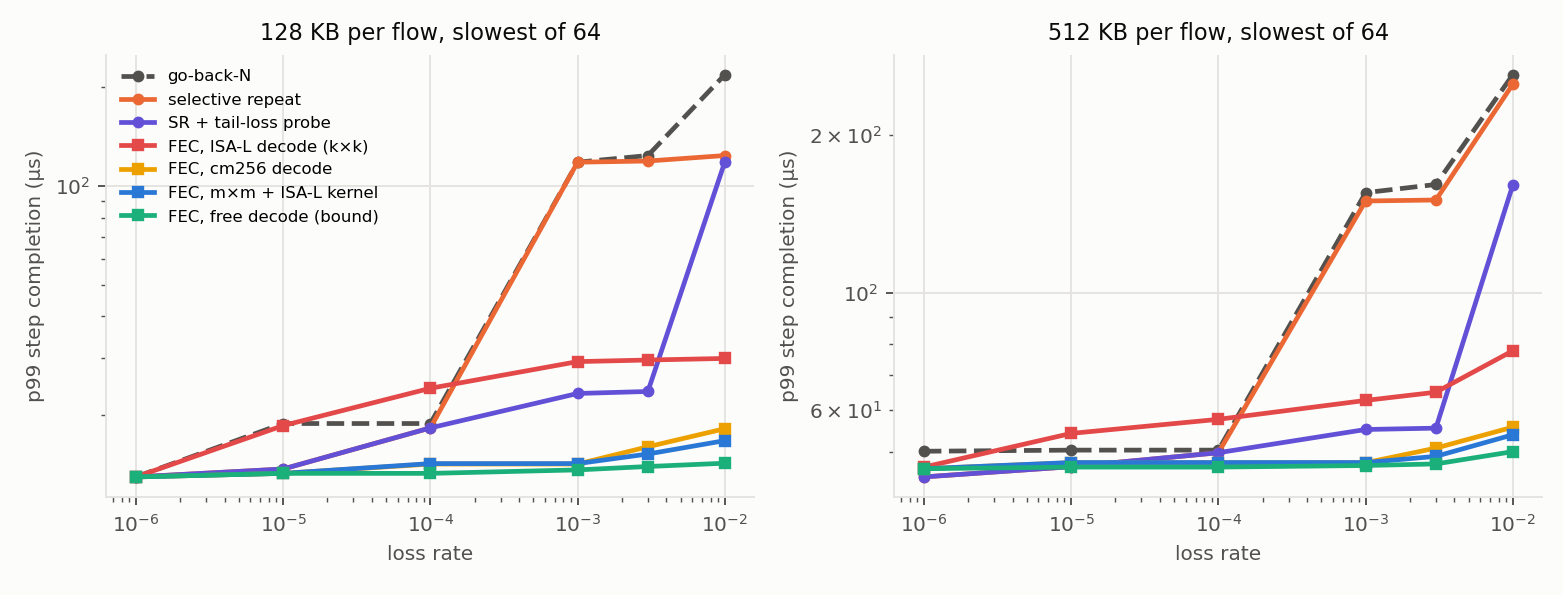
\includegraphics[width=\linewidth]{fig3_collective.png}
\caption{p99 completion of a 64-flow collective step versus loss rate (RTT 5\,\textmu s, 100\,Gbps).}
\label{fig:collective}
\end{figure}

\begin{figure*}[t]
\centering
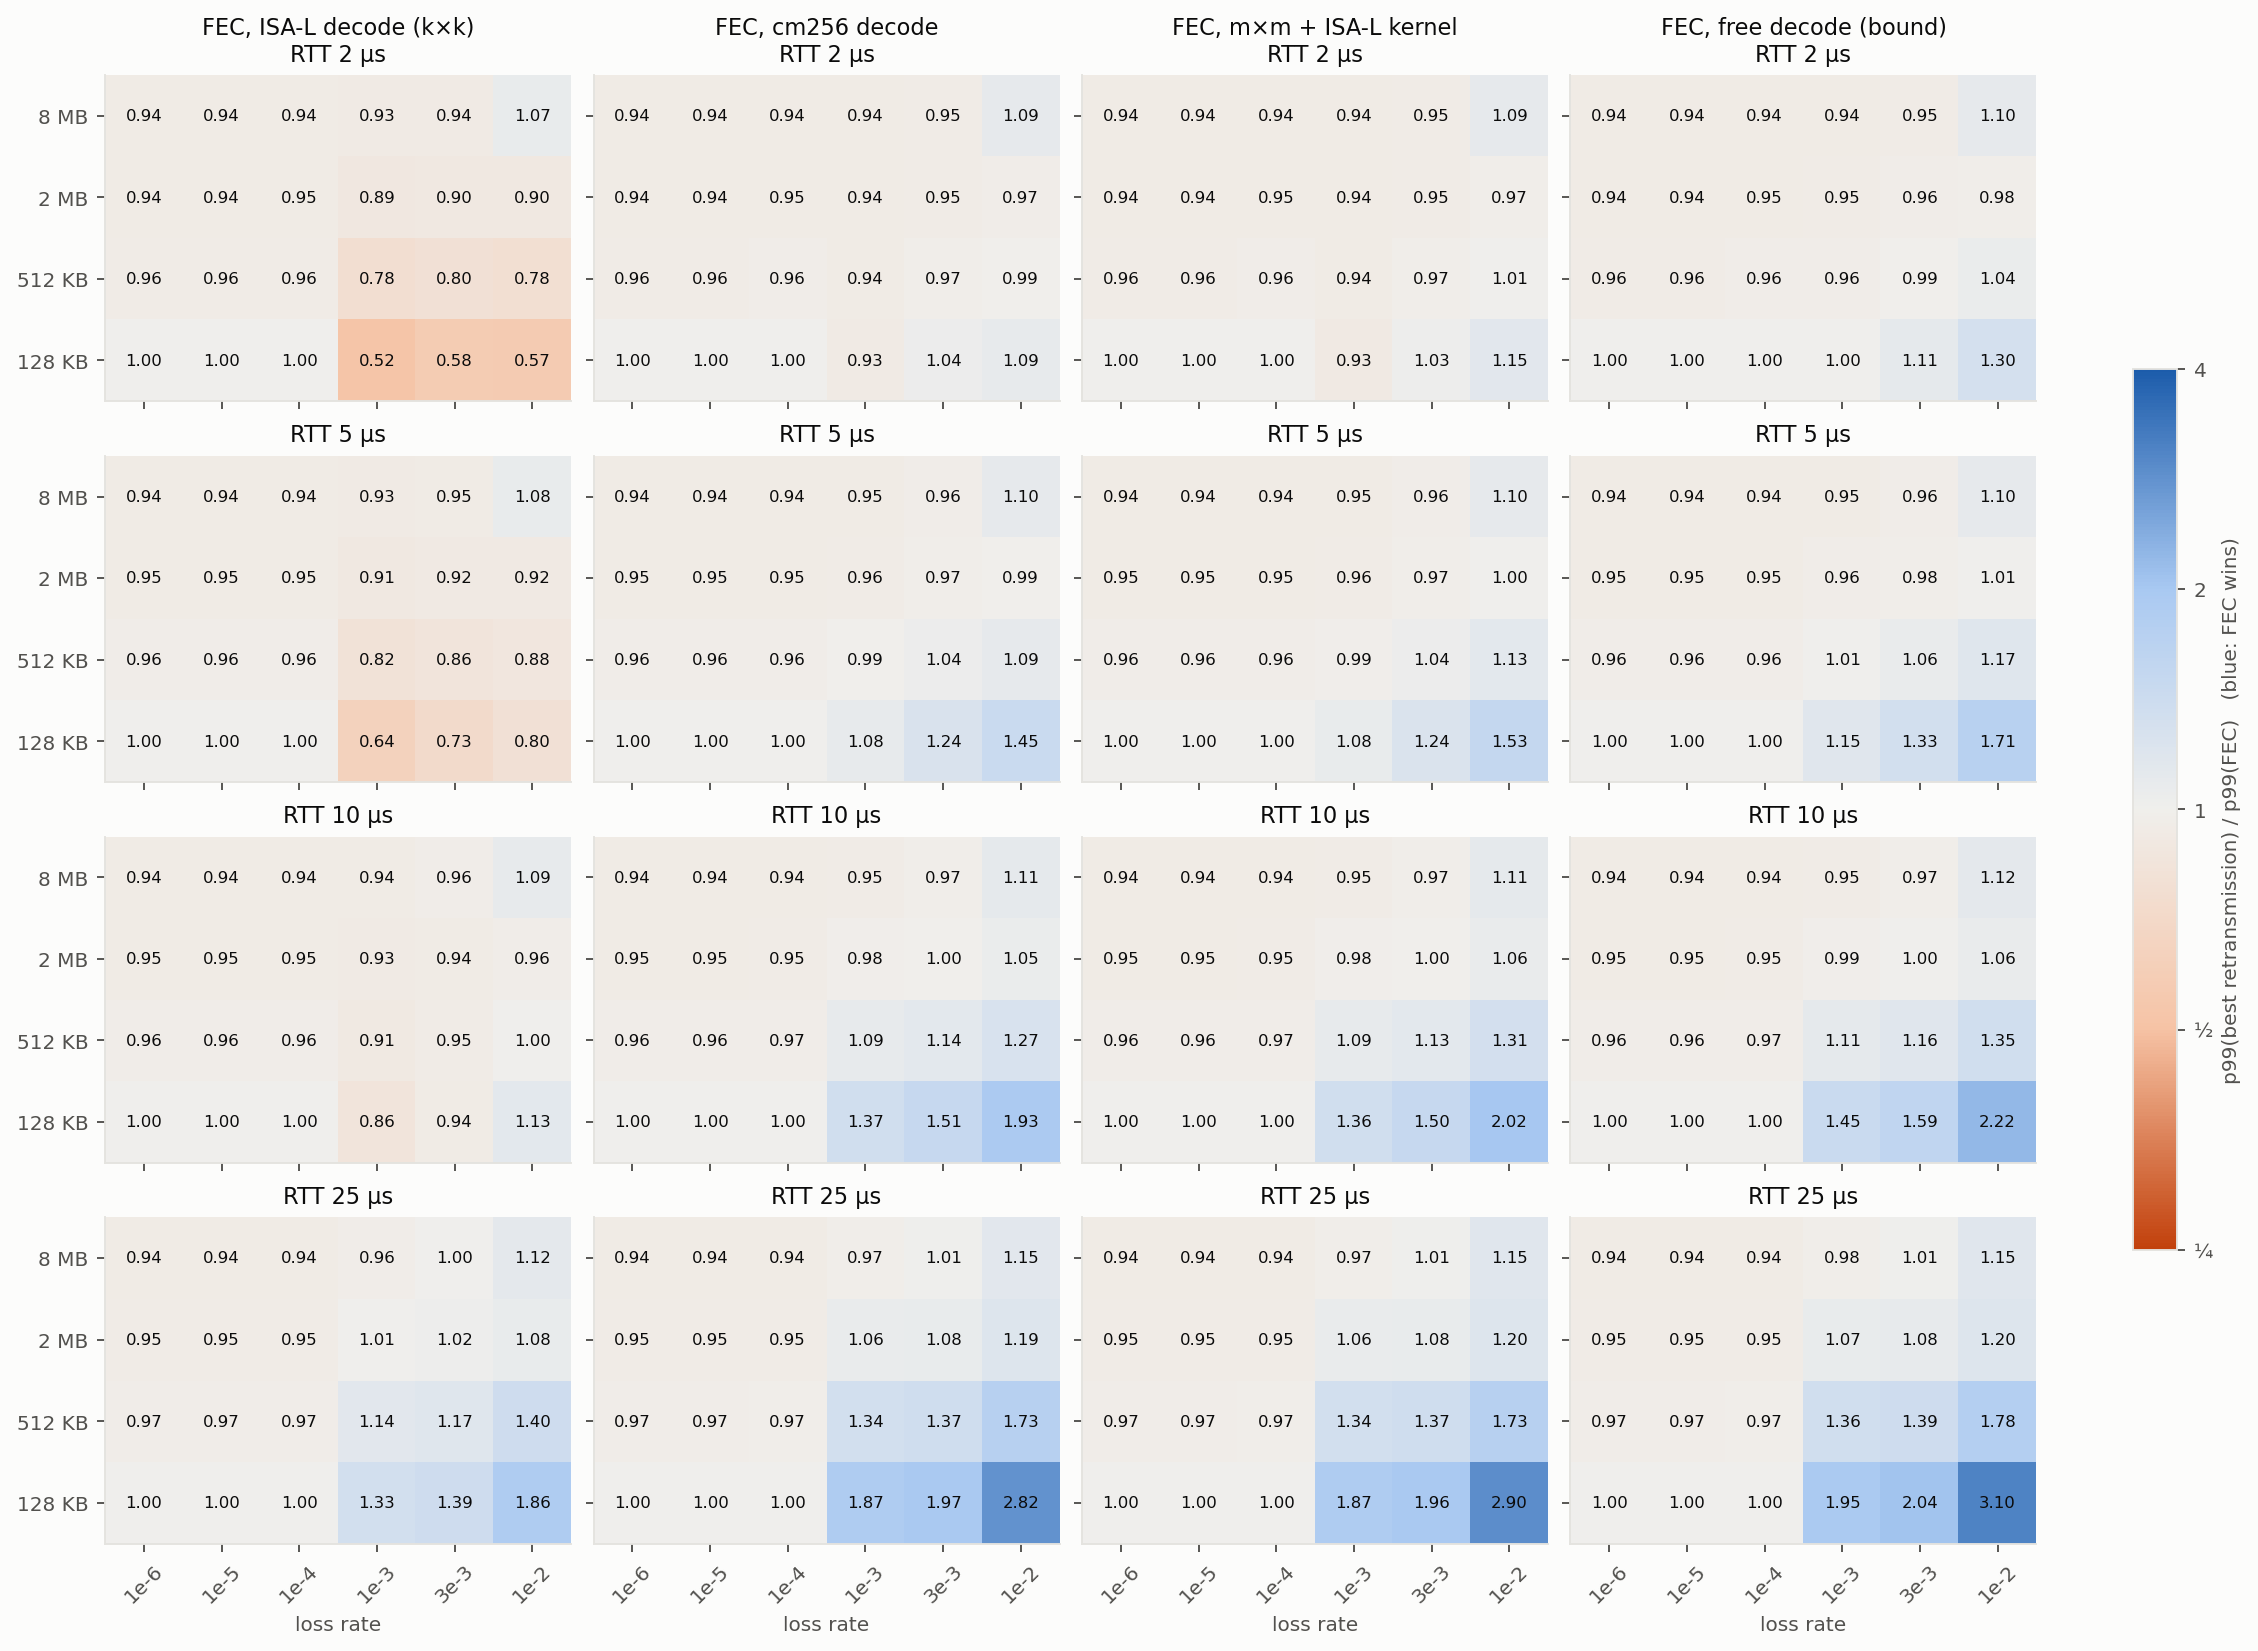
\includegraphics[width=\linewidth]{fig1_ratio_bernoulli.png}
\caption{p99(best retransmission)\,/\,p99(best FEC code) for a single flow, over loss rate and message
size. Rows are RTTs and columns are decoders. Blue means FEC wins.}
\label{fig:ratio}
\end{figure*}

\subsection{Limitations}
Our model has no congestion control, PFC or NIC pipeline. The flows in a collective step are
independent and do not share a bottleneck, the sender is not window-limited, and acknowledgements
are never lost. Decode costs come from one laptop CPU under WSL2. Losses are i.i.d.; our bursty
three-state model is not yet fitted to measured traces. Commodity RoCE timeouts are often far above
100\,\textmu s, which would favour FEC and SR+TLP further.


\section{Discussion}
\label{sec:discussion}

\paragraph{What a designer should take away.} FEC is worth its bandwidth for small messages and
collective steps at loss rates of $10^{-4}$ and above, but only with a decoder whose cost does not
grow with $k^3$. Off-the-shelf use of ISA-L's documented decode path is enough to turn a 1.6$\times$
win into a 2.1$\times$ loss at RTT 5\,\textmu s. Caching decode matrices recovers most of ISA-L's
cost when loss patterns repeat. Erasure-count decoding makes a cache miss cost about the same as a
hit, which matters because a code such as RS(36,32) has tens of thousands of distinct loss
patterns.

\paragraph{What is missing.} Our results come from simulation with measured decode costs, not from
an RDMA testbed. Flows in a collective step are independent, so they do not share incast bursts
or a bottleneck queue. The in-burst loss rate in our calibrated model is swept, not measured.
A NIC-offloaded decoder would shift the boundary again. Hardware validation is the obvious next
step.

\section{Conclusion}

At microsecond RTTs, whether erasure coding beats retransmission for RDMA depends less on the code
than on the decoder. With ISA-L's $k\times k$ decode path, FEC loses to selective repeat with a
tail-loss probe; with erasure-count decoding, a known but not universally implemented technique,
it wins by up to $3\times$ on collective steps and comes within 5--8\% of free decoding. The
benchmark, simulator and all scripts that produce our figures are available at
\url{https://github.com/1brahim74/thesis}.

\bibliographystyle{plain}
\bibliography{refs}

\end{document}
